\section{Complex optimisation}
\label{sec:Wirtinger}

Given a set of cross correlations between antenna voltages (the
visibility set) in a given time-frequency domain and a model of the sky brightness, the calibration
step in radio interferometry consists in estimating a set of
direction-dependent Jones matrices per antenna. This is usually done
using a chi-square minimisation technique such as the
Levenberg-Maquardt. In this paper, we use the alternative Wirtinger's
definition of complex derivative, instead of what is usually done by
considering the real and imaginary (later referred as the
{\it Wirtinger} and {\it classical} approaches respectively).

\subsection{RIME formalism}

Using the Radio Interferometry Measurement Equation (RIME) formalism
\citep[][]{Hamaker96}, the
4-polarisation visibility vector $\vbl$ measured on baseline $(pq)$,
at time $t$ and frequency $\nu$ can be written as


\begin{alignat}{2}
\label{eq:ME}
\vbl=&\text{Vec}\left(\Vbl\right)&\\
=&\displaystyle\sum\limits_{d} \left(\conj{\JMat^{d}_{qt\nu}}\Kron \JMat^{d}_{pt\nu}\right)
\text{Vec}\left(\Skyd\right) k^{d}_{(pq)t\nu}\\
\text{with}\ k^{d}_{(pq)t\nu}=&\exp{\left(-2 i\pi
  \left(\u\l+\v\m+\w\left(\text{n}-1\right)\right)\right)}\\
\text{and}\ \n=&\sqrt{1-\l^2-\m^2}
\end{alignat}

\noindent where $\JMat^{d}_{pt\nu}$ is the Jones matrix of antenna $p$
in direction $d$, $\Skyd$ is the four-polarization sky matrix, $\Kron$
is the Kronecker product, $[\u,\v,\w]^T$ is the baseline vector between antennas
$p$ and $q$ in wavelength units, and
$\vec{s}_d=[\l,\m,\n=\sqrt{1-\l^2-\m^2}]^T$ is a sky direction later
labeled as $d$.
In the following, the Jones matrix $\JMat^{d}_{pt\nu}$ is
represented by scalars $g^{d}_{pt\nu,k}$ as

\begin{equation}
\JMat^{d}_{pt\nu}=
\begin{bmatrix}
g^{d}_{pt\nu,0} & g^{d}_{pt\nu,2} \\ 
g^{d}_{pt\nu,1} & g^{d}_{pt\nu,3} 
\end{bmatrix}
\end{equation}

\noindent and the set of Jones matrices is represented by a gain
vector $\vec{g}$ containing the scalars $g^{d}_{pt\nu,k}$ for all
directions, antennas and polarisations.

From Eq. \ref{eq:ME}, the $i^{th}$ polarisation component of $\vbl$
can be written as

\begin{alignat}{2}
\label{eq:hpq}
\mathrm{v}^i_{pqt\nu}=&h^i_{pq}(\vec{g})\\
=&
\displaystyle\sum\limits_{d}
\displaystyle\sum\limits_{j=0}^3 \left(g^{d}_{pt\nu,\textbf{A}_{ij}}.\conj{g^{d}_{qt\nu,\textbf{B}_{ij}}}\right).k^{d}_{pqt\nu}.\text{s}_{d,j}
\end{alignat}

\noindent where 

\begin{equation}
\textbf{A}=
\begin{bmatrix}
0 & 2 & 0 & 2 \\ 
1 & 3 & 1 & 3 \\ 
0 & 2 & 0 & 2 \\
1 & 3 & 1 & 3 
\end{bmatrix}
\text{ and }
\textbf{B}=
\begin{bmatrix}
0 & 0 & 2 & 2 \\ 
0 & 0 & 2 & 2 \\ 
1 & 1 & 3 & 3 \\
1 & 1 & 3 & 3 
\end{bmatrix}
\end{equation}



\subsection{Wirtinger complex derivative}
\label{sec:Cderiv}

In order to compute a Jacobian, a
derivative definition for complex numbers has to be chosen. Instead of
differentiating against real and imaginary parts independently, one can
adopt a Wirtinger differentiation point of view and consider the
complex and their conjugate as being independent. Choosing this type of differentiation
turns out to be rather powerful to solve problems of the form of
Eq. \ref{eq:ME} (see
Sec. \ref{sec:Solver}). If a complex number is written as $z=x+iy$, the
Wirtinger complex derivative operator becomes


\begin{alignat}{3}
\frac{\partial }{\partial z}&=&\frac{1}{2}\left(\frac{\partial }{\partial x}-i\frac{\partial }{\partial y}\right)\\
\text{and }\frac{\partial }{\partial \conj{z}}&=&\frac{1}{2}\left(\frac{\partial }{\partial x}+i\frac{\partial }{\partial y}\right)
\end{alignat}

\noindent where $x$ and $y$ are the real and imaginary parts
respectively. The
Wirtinger has a trivial but remarkable property that a scalar and its
complex conjugate can be viewed as independent variables, and in
particular

%% \begin{alignat}{3}
%% \label{eq:propConj}
%% \frac{\partial \conj{z}}{\partial z}&=&0
%% \end{alignat}

\begin{equation}
\label{eq:propConj}
\frac{\partial \conj{z}}{\partial z}=0
\text{ and }
\frac{\partial z}{\partial \conj{z}}=0
\end{equation}


Considering the sky, gain, and geometry relation given in
Eq. \ref{eq:ME}, according to the property of Wirtinger derivative of complex
conjugate (Eq. \ref{eq:propConj})

\begin{alignat}{3}
\label{eq:Deriv_gp}
\frac{\partial \mathrm{v}^i_{pqt\nu}}{\partial g^{d}_{pt\nu,\textbf{A}_{ij}}}=&
\left(\conj{g^{d}_{qt\nu,\textbf{B}_{ij}}}\text{s}_{d,j}\right).k^{d}_{pqt\nu}\\
\label{eq:Deriv_gq}
\text{and}\ 
\frac{\partial \mathrm{v}^i_{pqt\nu}}{\partial g^{d}_{qt\nu,\textbf{B}_{ij}}}=&0
\end{alignat}

\noindent while differentiating against the complex conjugate of those
variables, one obtain

\begin{alignat}{3}
\label{eq:Deriv_Cgp}
\frac{\partial \mathrm{v}^i_{pqt\nu}}{\partial \conjp{g^{d}_{pt\nu,\textbf{A}_{ij}}}}=&0\\
\label{eq:Deriv_Cgq}
\text{and}\ 
\frac{\partial \mathrm{v}^i_{pqt\nu}}{\partial \conjp{g^{d}_{qt\nu,\textbf{B}_{ij}}}}=&
\left(g^{d}_{pt\nu,\textbf{A}_{ij}}\text{s}_{d,j}\right).k^{d}_{pqt\nu}
\end{alignat}

Interestingly, Eq. \ref{eq:Deriv_gp},
\ref{eq:Deriv_gq}, \ref{eq:Deriv_Cgp} and \ref{eq:Deriv_Cgq} show that the
derivatives are always constant with respect to the differential
variable.

\subsection{Wirtinger Jacobian}
\label{sec:WirtingerJacob}

This section describes the structure of the Wirtinger Jacobian $\JV$ using the
results of Sec. \ref{sec:Cderiv}.
First, let consider the visibility vector $\vbl$
for all given time frequency blocks, and write the antenna,
polarisation, and direction dependent gain vector as
$\vec{g}$. Its size is $4n_an_d$, and have for $k^{th}$ component
$k=j+4\times d+4\times a \times n_d$ the gain of antenna $a$ in
direction $d$ for polarisation $j$, where $n_a$, and $n_d$ are the
number of antenna and directions.

The corresponding Wirtinger Jacobian $\JVpq$ has size $(4n_t n_{\nu})\times (8n_a n_d)$ ($n_t$
and $n_{\nu}$ are the number of time and frequency points), and can be
decomposed as follows:

\begin{alignat}{2}
\label{eq:dV}
\dbf\vbl=&\JVpq\ \dbf\gwirt\\
=&\JVpqg\ \dbf\g+\JVpqCg\ \dbf\conj{\g}\\
\text{where }\dgwirt=&
\begin{bmatrix}
\dbf\vec{g}\\
\dbf\conj{\vec{g}}
\end{bmatrix}\\
\text{and }\JVpq=&
\begin{bmatrix}
\JVpqg & \JVpqCg
\end{bmatrix}
\end{alignat}

%% The visibility vector $\textbf{v}_{(pq)}$ has to be
%% differentiated on the complex conjugate as well, so in the following we write the
%% Wirtinger gain vector $\bm{g_{\!_{W}}}$ and its differencial element as:

%% %\begin{equation}
%% %\bm{g_{W}}=

%% \gwirt=
%% \begin{bmatrix}
%% \vec{g}\\
%% \conj{\vec{g}}
%% \end{bmatrix}
%% \text{ and }
%% %\end{equation}




Each cell of
$\JVpq$, $\JVpqg$ and $\JVpqCg$ can be written using Eq. \ref{eq:Deriv_gp}, \ref{eq:Deriv_gq},
\ref{eq:Deriv_Cgp} and \ref{eq:Deriv_Cgq}. Specifically, line corresponds to a
single $i$-polarisation measurement at $(t\nu)$ for the $(pq)$ baseline, and a column
$j+4d+a.4n_d$ to a gain for polarisation $j$, antenna $a$ and
direction $d$ ($g^{d}_{a,j}$). The matrix $\JVpq$ can be described as


%% \begin{alignat}{2}
%% \mathcal{J}\left(\textbf{V}_{(pq)}\right)=&caca\\
%% \end{alignat}


\begin{alignat}{2}
\label{eq:Jpq0}
\left[\JVpqg\right]_{t\nu,i}=&
\begin{cases}
\left(\conj{g^{d}_{qt\nu,\textbf{B}_{ij}}}\text{s}_{d,j}\right).k^{d}_{pqt\nu}\text{ for }a=p\\
0\ \text{otherwise}
\end{cases}
\end{alignat}

\noindent and

\begin{alignat}{2}
\label{eq:Jpq1}
\left[\JVpqCg\right]_{t\nu,i}=&
\begin{cases}
\left(g^{d}_{pt\nu,\textbf{A}_{ij}}\text{s}_{d,j}\right).k^{d}_{pqt\nu}\text{ for }a=q\\
0\ \text{otherwise}
\end{cases}
\end{alignat}

\noindent One can see that non-zero columns are the ones
corresponding to all direction and all polarisations for antenna $p$. The Jacobian for all
baselines is written in a similar way, by superposing the
$\JVpq$ for all $(pq)$ pairs as follows:

\begin{alignat}{2}
\label{eq:J}
\JV=&
\begin{bmatrix} 
\vdots \\ 
\JVpq\\ 
\vdots \\ 
\end{bmatrix}
\end{alignat}

\noindent which have size $[(4n_{bl} n_t n_{\nu})\times (8n_a n_d)]$,
where $n_{bl}$ is the number of baselines and is typically
$n_{bl}=n_a(n_a-1)/2$. Although it has large dimensions, $\JV$ is
sparse.



%% \begin{figure*}[ht!]
%% \begin{center}
%% %\hspace*{-1.3cm}
%% \includegraphics[width=17cm]{resid}
%% 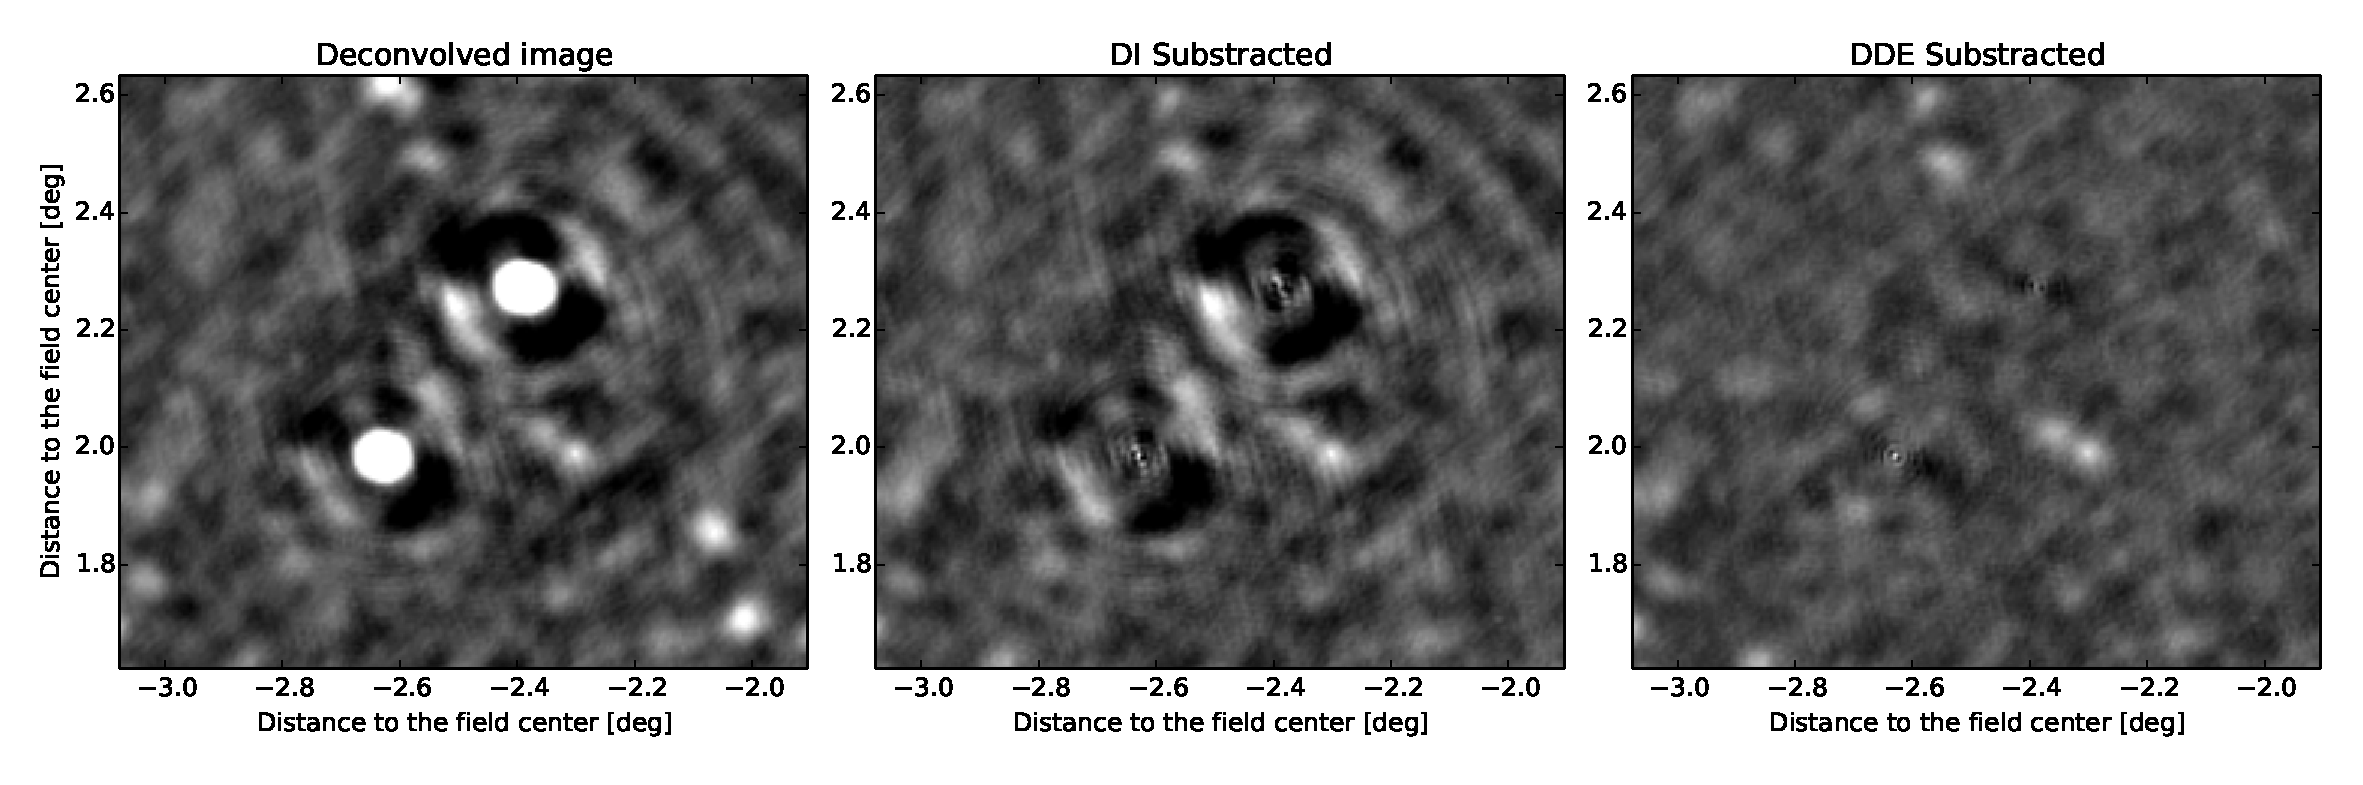
\includegraphics[width=17cm]{residZoom}
%% \caption{\label{fig:resid} This figure shows compares the image
%%   (left), the residuals data after simple skymodel substraction
%%   (center), and the residuals data after substracting the
%%   sky model corrupted by the direction-dependent solution (right).}
%% \end{center}
%% \end{figure*}

